\documentclass{article}
\usepackage{amsmath,amssymb}
\usepackage{tikz}
\usetikzlibrary{arrows.meta,positioning,calc,shapes.geometric}
\pagestyle{empty}
\begin{document}
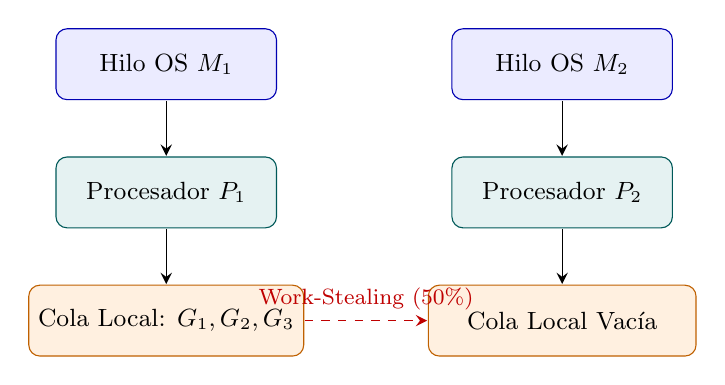
\begin{tikzpicture}
\tikzset{node distance=1.6cm, >=stealth, thick, font=\small}
\node[draw=blue!70!black, fill=blue!8, rounded corners, minimum width=2.8cm, minimum height=0.9cm, align=center] (m1) {Hilo OS $M_1$};
\node[draw=teal!70!black, fill=teal!10, rounded corners, minimum width=2.8cm, minimum height=0.9cm, align=center, below=0.7cm of m1] (p1) {Procesador $P_1$};
\node[draw=orange!75!black, fill=orange!12, rounded corners, minimum width=3.4cm, minimum height=0.9cm, align=center, below=0.7cm of p1] (q1) {Cola Local: $G_1, G_2, G_3$};
\node[draw=blue!70!black, fill=blue!8, rounded corners, minimum width=2.8cm, minimum height=0.9cm, align=center, right=2.2cm of m1] (m2) {Hilo OS $M_2$};
\node[draw=teal!70!black, fill=teal!10, rounded corners, minimum width=2.8cm, minimum height=0.9cm, align=center, below=0.7cm of m2] (p2) {Procesador $P_2$};
\node[draw=orange!75!black, fill=orange!12, rounded corners, minimum width=3.4cm, minimum height=0.9cm, align=center, below=0.7cm of p2] (q2) {Cola Local Vacía};
\draw[->] (m1) -- (p1);
\draw[->] (p1) -- (q1);
\draw[->] (m2) -- (p2);
\draw[->] (p2) -- (q2);
\draw[->, dashed, red!75!black] (q1.east) -- node[above, font=\footnotesize] {Work-Stealing ($50\%$)} (q2.west);
\end{tikzpicture}
\end{document}
